%-----------------------------------LICENSE------------------------------------%
%   This file is part of tikz_figures.                                         %
%                                                                              %
%   tikz_figures is free software: you can redistribute it and/or              %
%   modify it it under the terms of the GNU General Public License as          %
%   published by the Free Software Foundation, either version 3 of the         %
%   License, or (at your option) any later version.                            %
%                                                                              %
%   tikz_figures is distributed in the hope that it will be useful,            %
%   but WITHOUT ANY WARRANTY; without even the implied warranty of             %
%   MERCHANTABILITY or FITNESS FOR A PARTICULAR PURPOSE.  See the              %
%   GNU General Public License for more details.                               %
%                                                                              %
%   You should have received a copy of the GNU General Public License along    %
%   with tikz_figures.  If not, see <https://www.gnu.org/licenses/>.           %
%------------------------------------------------------------------------------%

% Use the standalone class for displaying the tikz image on a small PDF.
\documentclass[crop, tikz]{standalone}

% Import the tikz package to use for the drawing.
\usepackage{tikz}

% Tikz libraries used in the drawing.
\usetikzlibrary{calc}

% Begin the document.
\begin{document}

    % Draw the figure.
    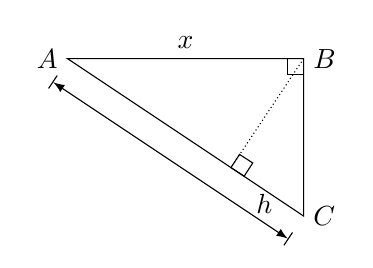
\begin{tikzpicture}

        % Positions for all of the points.
        \coordinate (A) at (0.0, 0.0);
        \coordinate (B) at (3.0, 0.0);
        \coordinate (C) at (3.0, -2.0);
        \coordinate (D) at ($(A)!(B)!(C)$);
        \coordinate (E) at ($(A)+(-123:0.35)$);
        \coordinate (F) at ($(C)+(-123:0.35)$);

        % Label the vertices of the triangle.
        \node at (A) [anchor = east] {$A$};
        \node at (B) [anchor = west] {$B$};
        \node at (C) [anchor = west] {$C$};

        % Label the lengths in the triangle.
        \node at (1.5, 0.0) [anchor = south] {$x$};
        \node at (2.5, -1.85) {$\small{h}$};

        % Draw the triangle.
        \draw (A) to (B) to (C) to cycle;

        % Square for the right angle at B.
        \draw (B) rectangle +(-0.2, -0.2);

        % Drop a perpendicular line from B onto AC.
        \draw [densely dotted] (B) to (D);

        % Draw a square for the right angle made with AC.
        \draw [rotate = -33] (D) rectangle +(0.2, 0.2);

        % Label the hypotenuse.
        \draw [|<->|, > = latex] (E) to (F);
    \end{tikzpicture}
\end{document}
